\documentclass[sigconf]{acmart}

\usepackage{url}

\newcommand{\ts}{\textsuperscript}

\begin{document}

\title{Reproduce Stock Price Prediction Tasks with News Analysis}
\subtitle{NYU FRE-7871 Final Project Report}

\author{Pei-Lun Liao}
\affiliation{%
  \institution{New York University}
}
\email{pll273@nyu.edu}

\begin{abstract}
In this project \footnote{The source code was released on https://github.com/plliao/FRE-7871-project}, selected related works will be reproduced with different financial news dataset. The goal is to understand techniques and challenges in stock price prediction.
\end{abstract}
\maketitle

\section{Introduction}
Nowadays, traders apply machine learning technique to extract information from financial news data. The information can be used to boost the accuracy of stock price
prediction \cite{AZFinText, Ding2014, Ding2015}. The project aims to reproduce selected related works \cite{AZFinText}. Hence, people can learn the challenge and technique
that are crucial in stock price prediction.

\section{Approaches}
\subsection{Data}
Data quality is crucial to make the accurate prediction \cite{stanford}. Unfortunately, it is not easy to find a publicly available financial news dataset. For example, the public financial
news dataset published in \cite{Ding2014} was currently unavailable due to license issue \cite{fn}. Another corpus available online requires membership and subscription fee \cite{nyt}.
Also, it is not practical to crawl dataset from business news media in this one month project. Most of the time will be spent on data collecting, cleaning, and processing instead of
understanding the technique that works for stock price prediction.

\subsubsection{Webhose.io and IEX API}
Fortunately, an available financial news dataset was found on Webhose.io \cite{data}. The data was crawled from the Internet from July to October in 2015. 47,851 news articles were collected
in machine-readable format. However, there is no paper shows the dataset could help stock price prediction. We filtered new articles by finding the S \& P 500 company name in the article as
described in section \ref{ticker_labeling}. After that, we have 5,375 articles left.

News articles from Webhose.io come globally as shown in Figure \ref{fig:web_contry} and \ref{fig:web_site}. Each day we have around 50 articles as shown in Figure \ref{fig:web_per_day}.
Generally, more than half of the news was published after the close time.

End of date S \& P 500 stock prices from July to October in 2015 was downloaded from IEX API \cite{IEX}. However, we can't find the S \& P 500 stock price by minutes. Therefore, we could not
have the current stock price to predict the next 20 minutes stock price as the experiment in AZFinText. What we can do is to predict the trend between the open time and close time and to see
if we can capture some text pattern.

\begin{figure}
  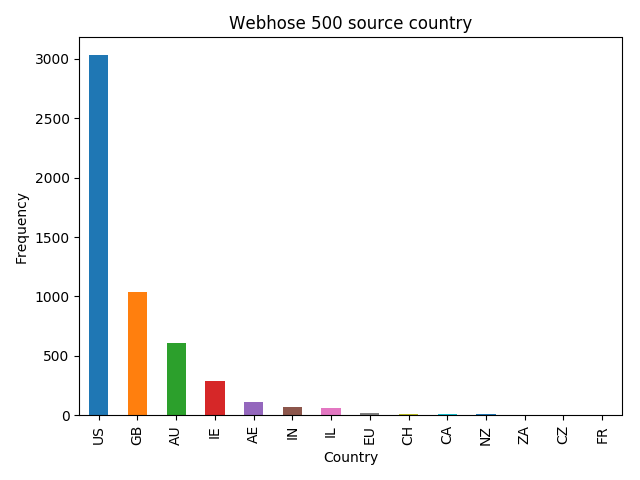
\includegraphics[width=\linewidth]{../../picture/webhose_500_country.png}
  \caption{Webhose.io with S \& P 500 news article country source}
  \label{fig:web_contry}
\end{figure}

\begin{figure}
  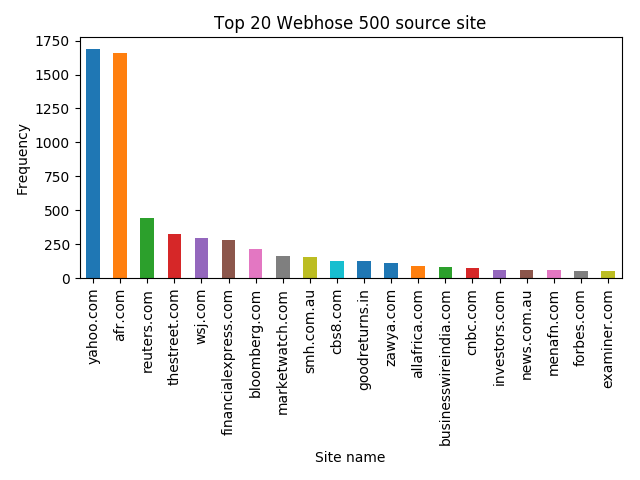
\includegraphics[width=\linewidth]{../../picture/webhose_500_site.png}
  \caption{Webhose.io with S \& P 500 news article site source}
  \label{fig:web_site}
\end{figure}

\begin{figure}
  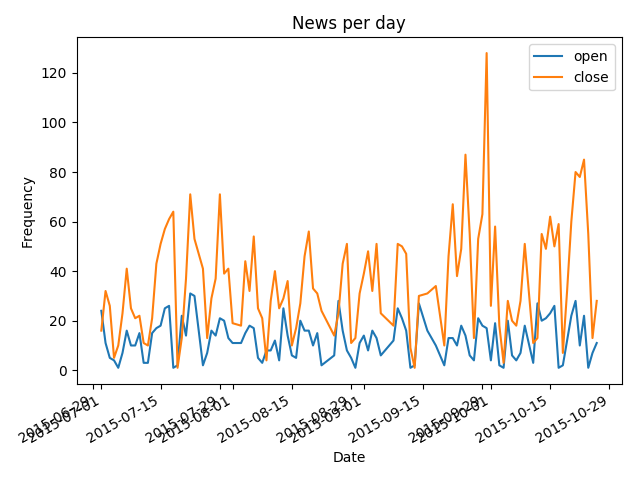
\includegraphics[width=\linewidth]{../../picture/webhose_500_news_per_day.png}
  \caption{Webhose.io S \& P 500 news per day}
  \label{fig:web_per_day}
\end{figure}

\subsubsection{Reuters and IEX API}
Due to the quality issue in Webhose.io dataset, we need to find another way to experiment. Hence, we crawled S \& P 500 stock prices by minute from IEX API \cite{IEX} and collected 9013 business news articles
from Reuters \cite{reuters} in the period between July 2\ts{nd} 2018 to September 30\ts{th} 2018. Due to the limited available open stock price data, I can only collect three months dataset. The data quality is not
guaranteed as well. Finally, 1107 articles can be mapped to a specific stock name, and only 308 articles were published in open trading time. Each day, we have around 15 articles as shown in Figure \ref{fig:re_per_day}.

\begin{figure}
  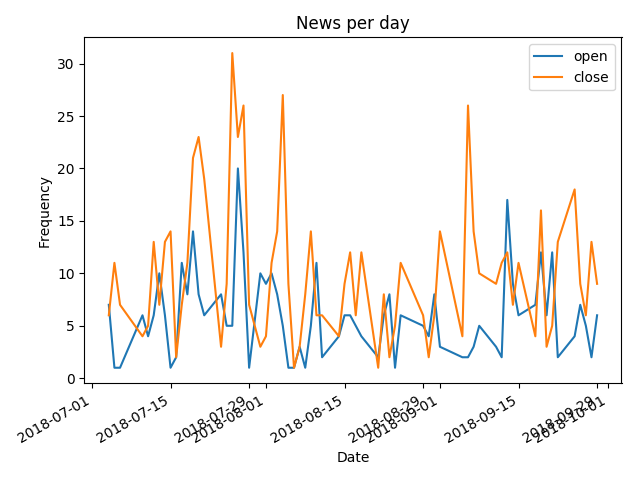
\includegraphics[width=\linewidth]{../../picture/reuter_news_per_day.png}
  \caption{Reuters S \& P 500 news per day}
  \label{fig:re_per_day}
\end{figure}


\subsection{Tickers labeling} \label{ticker_labeling}
We cleaned S \& P 500 company names by removing punctuations and common terms like "Inc.", "Corp.", or ".com" and mapped an article to the stock if we can find the name in the article. Also, some formal
company name like "Alphabet Class A" and "Alphabet Class C" were replaced to "Google" since reporters often use the word "Google" instead of "Alphabet" in their articles. We removed the terms like "Google+"
and "Google Plus" to get rid of the sharing on social media text. We ignore the ambiguous company name for data quality as well. For example, "CA, Inc." was ignored because the word "CA" is ambiguous in an article.

The distribution of tickers on Webhose.io and Reuters dataset can be found in Figure \ref{fig:web_ticker} and \ref{fig:re_ticker}. Google contributes the most news articles in both Webhose.io and Reuters dataset.
In this process, we found several company names can be mentioned in the same article. Hence, we will have the same text features with different label price. Sometimes, people will mention rival companies in the
same article \cite{stanford} and the article will describe good and bad things at the same time. It will hurt our performance. The better way to do that is identifying the company mentioned in a sentence and
collecting those sentences into an article. However, we didn't implement that.


\begin{figure}
  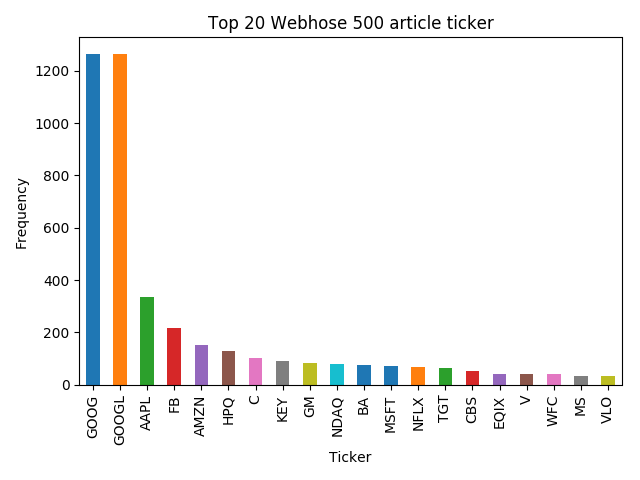
\includegraphics[width=\linewidth]{../../picture/webhose_500_ticker.png}
  \caption{Top 20 S \& P 500 tickers in Webhose.io dataset}
  \label{fig:web_ticker}
\end{figure}

\begin{figure}
  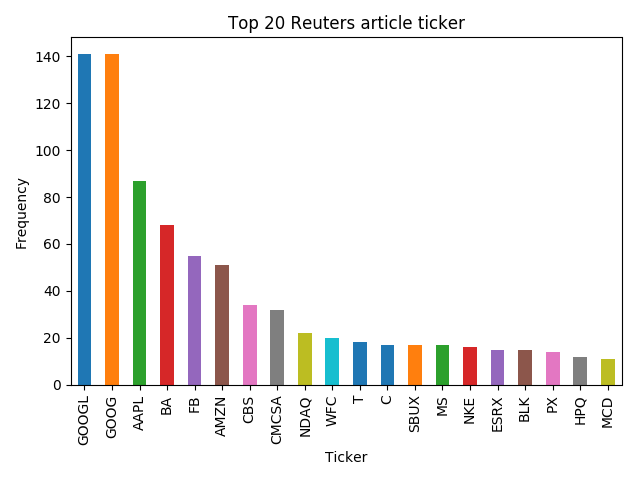
\includegraphics[width=\linewidth]{../../picture/reuter_ticker.png}
  \caption{To 20 S \& P 500 tickers in Reuters dataset}
  \label{fig:re_ticker}
\end{figure}

\subsection{Price Labeling}
For each news article, we attached prices by the ticker name we found.

\subsubsection{Webhose.io and IEX API}
Since we didn't have the stock price by minutes, we attached the prices we have before and after the news published. For example, assume the stock market is open on 10/01. The news published at 10:00 on 10/01
will be attached the prices at 09:30 and 16:00 on 10/01. It is the open and close price on 10/01. We are interested in the news relationship with the market price. For the same reason, if the
article published at 19:00 on 10/01, we will attach the close price at 16:00 on 10/01 and the open price at 09:30 on 10/02 to the article. After that, Webhose.io dataset has 4074 articles left.

\subsubsection{Reuters and IEX API}
For the articles on Reuters, since we have the stock price by minutes, we attached the next 20 minutes price if the price existed. For example, assume the stock market is open on 10/01. The news published at 10:00
on 10/01 will be attached to the high market price at 10:00 and the low market price at 10:20 on 10/01. We choose 20 minutes as the same setting in  AZFinText \cite{AZFinText}. The reason for selecting the high market
price at the published time and the low market price next 20 minutes is that I assume we at least could buy the stock with highest market price and sell it with the lowest market price. If the article published at 15:45
or 09:10 on 10/01, since the stock is not open or close, we ignore the news. Finally, we have 308 articles left. The amount of data is also insufficient, and the experiment result may not be convincing.

\subsection{Original Plan} \label{plan}
\subsubsection{Stage 1: bag-of-words}
	The goal in stage 1 is reproducing the experiment result in AZFinText system \cite{AZFinText}. AZFinText represented article in the bag-of-words with only proper nouns. The datasets were Yahoo Finance news 
	articles and the S \& P 500 index. Reproducing the experiment in AZFinText can prove that the data from Webhose.io or Reuters also works for stock price prediction. Moreover, we examined whether only using 
	proper nouns helps the performance.

	The experiment setup will follow the AZFinText paper. We will represent articles in the bag-of-words and use SVR to predict stock price. Finally, we evaluate the result by the rate of return.
	The strategy is buying the stock as the predicted price is greater than or equal to 1\% movement from the stock price at the time the article was released. Then, sell the stock after 20 minutes.
	In stage 1, we will have four different results to compare.
	\\
	\begin{itemize}
		\item 1. Stock price
		\item 2. Stock price + News in bag-of-words
		\item 3. Stock price + News in bag-of-words without stopwords
		\item 4. Stock price + News in bag-of-words with only proper nouns
	\end{itemize}
	The expected performance will be 4 > 3 > 2 > 1 as the paper described.

\subsubsection{Stage 2: word and sentence representation}
	In this stage, We are curious how modern deep learning techniques like word2vec, seq2seq, and CNN-LSTM language models could help improve the performance.  
	\begin{itemize}
		\item 5. Stock price + News feature in average word2vec \cite{word2vec1, word2vec2}
		\item 6. Stock price + News feature in Skip-Thought vector\cite{skip}
		\item 7. Stock price + News feature in CNN-LSTM encoding \cite{CNN2RNN} (may try to find pre-trained model)
	\end{itemize}
	The performance in stage 2 should be better than the one in stage 1.

\section{Experiment}
\subsection{Data processing}
We remove stop words, punctuation, number, low-frequency words, and high-frequency words in the article. The threshold of the low and high frequency are 10 and 100
for the Webhose.io dataset and 5 and 50 for the Reuters dataset.

\subsection{Tasks}
We have three different tasks. The classification task is to predict if the price goes up. The regression problem is to predict the price difference. The final one is applying a simple strategy to see what we can
gain. The strategy is trading as the predicted price difference is positive. We use logistic regression, ridge regression, and SVR in the experiment.
\begin{itemize}
	\item Classification task: close price goes up or down
	\item Regression task: close and open price difference
	\item Trading strategy task: compute return using the prediction price
\end{itemize} 
The reason not using the same strategy as in AZFinText is for all models we could not have 1 \% return. Hence, we have 0 return rate for all models and features.
So the result is not comparable as well. Hence, we start with a more straightforward strategy.

\subsection{Features}
We experiment five different features on our tasks. Most of the features are described in section \ref{plan}. However, I didn't use stock price features in the experiment.
The idea is to see how good a text feature can contribute.
\begin{itemize}
	\item Bag-of-words: The bag-of-words features are the words count with L2 norm normalization. We tried the bag-of-words with and without stop words. We also experimented using bag-of-words with tri-gram.
	\item Bag-of-words with pos tag filtering: We tag our words using NLTK \cite{nltk} and only pick the words in the selected tags. We explore several different settings as below.
		\begin{itemize}
			\item Proper noun: ['NNP', 'NNPS']
			\item Noun: ['NNP', 'NNPS', 'NN', 'NNS']
			\item Noun and verb: ['NNP', 'NNPS', 'NN', 'NNS', 'VB', 'VBD', 'VBG', 'VBN', 'VBP', 'VBZ']
			\item Noun and adj: ['NNP', 'NNPS', 'NN', 'NNS', 'JJ', 'JJR', 'JJS']
			\item Noun, verb, and adj: ['NNP', 'NNPS', 'NN', 'NNS', 'VB', 'VBD', 'VBG', 'VBN', 'VBP', 'VBZ', 'JJ', 'JJR', 'JJS']
		\end{itemize}
	\item tf-idf: We compute the tf-idf in our corpus without stopwords.
	\item Average word2vec: We use Gensim \cite{gensim} with two pretrain models, Glove\cite{glove} and Google word2vec\cite{word2vec1, word2vec2}. The word embedding size is 300.
	\item Skip-thought vector\cite{skip}: Only the first 100 words are feed to avoid zero embedding vector. I used two pretrained TensorFlow\cite{tf} model, unidirectional and bidirectional model\cite{skip} to generate the features.
	The feature size is 2400.
\end{itemize} 

\subsection{Evaluation}
Since the data is time series, we can't apply standard K-fold cross-validation to our model because we can have the forward bias. Hence, we use K fold time series cross-validation instead. We choose K as 5 for Reuters and K as 10 for
Webhose.io dataset. We built word dictionary and scaled our features only on the observable dataset. Then, we predict the dataset on the next fold. If there are new words in the article, we ignore them.
We evaluate accuracy for the classification task, mean square error for the regression task and return in dollar for trading strategy task.

\section{Result}
\subsection{Features comparison}
We evaluate the performance with different features. Figure \ref{fig:web_tr_cls_all} and \ref{fig:web_cls_all} show the result on Webhose.io dataset. We can found  bag-of-words and tf-idf feature outperform word embedding feautes
in training data. This because the the discrete word features often capture some specific words and the model will overfit on that words. Hence, we can find in Figure \ref{fig:web_cls_all} the discrete word features do not perform as it did
in training data. The word analysis on the model could be found in Figure \ref{fig:web_neg_rid} and \ref{fig:web_pos_rid}. In Figure \ref{fig:web_pos_rid}, we can see the term "Ruth Porat", CFO of Google, and "Jeff Bezos", CEO of Amazon
are two of the most important positive terms. This is because in July to Oct 2015 Google and Amazon's stock price grew a lot. Then, the model learned their names as positive term. However, it doesn't imply anything in the future. It is the reason
for the bad performance.

\begin{figure}
  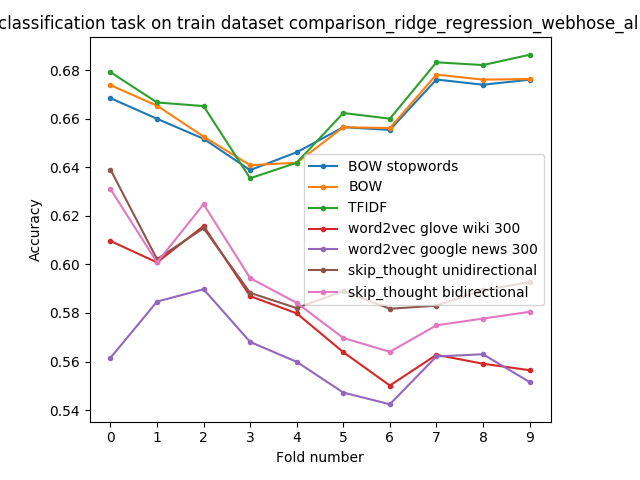
\includegraphics[width=\linewidth]{../../picture/experiment/classification_train_comparison_ridge_regression_webhose_all.png}
  \caption{Classification task on Webhose.io train data using Ridge regression}
  \label{fig:web_tr_cls_all}
\end{figure}

\begin{figure}
  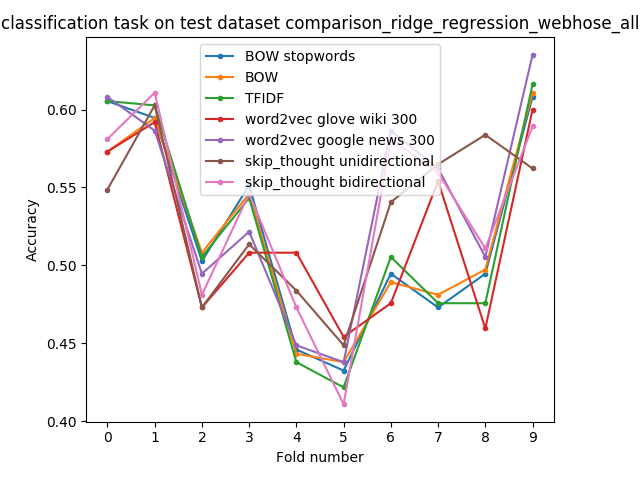
\includegraphics[width=\linewidth]{../../picture/experiment/classification_test_comparison_ridge_regression_webhose_all.png}
  \caption{Classification task on Webhose.io testing data using Ridge regression}
  \label{fig:web_cls_all}
\end{figure}

\begin{figure}
  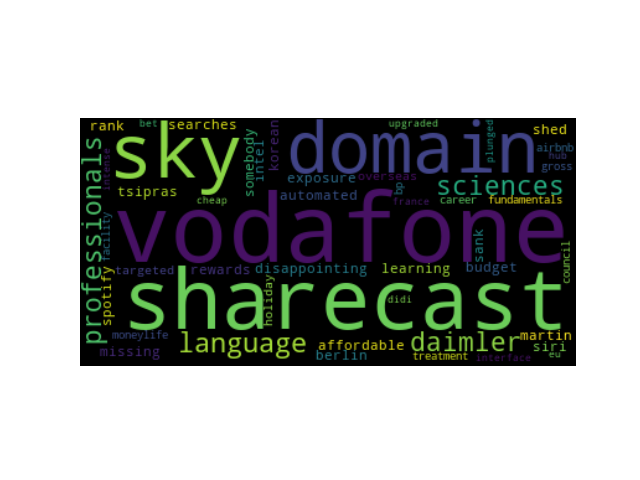
\includegraphics[width=\linewidth]{../../picture/wordCloud/ridge_regression_negative_(webhose,_bow_noun,_verb_and_adj).png}
  \caption{Negative terms on Webhose.io data by the weight of ridge regression}
  \label{fig:web_neg_rid}
\end{figure}

\begin{figure}
  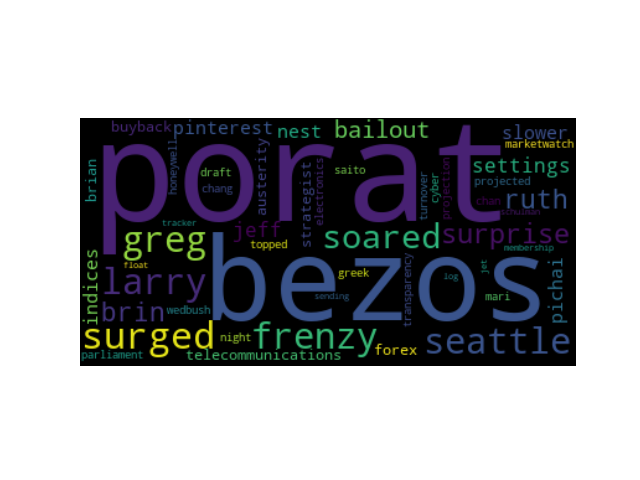
\includegraphics[width=\linewidth]{../../picture/wordCloud/ridge_regression_positive_(webhose,_bow_noun,_verb_and_adj).png}
  \caption{Positive terms on Webhose.io data by the weight of ridge regression}
  \label{fig:web_pos_rid}
\end{figure}

The result for Reuters can be found in Figure \ref{fig:re_tr_cls_all} and \ref{fig:re_cls_all}. There is not much difference between the features. Several reasons could cause it. For example, different companies share the same text feature as mentioned in section \ref{ticker_labeling} could make it happened. Insufficient data, 308 articles, can make things worse.

\begin{figure}
  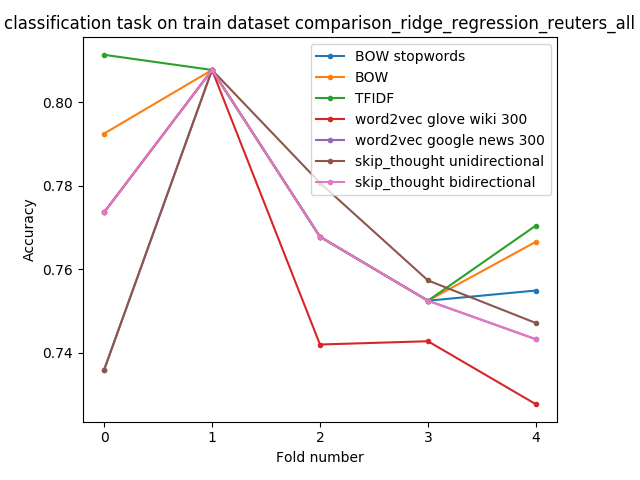
\includegraphics[width=\linewidth]{../../picture/experiment/classification_train_comparison_ridge_regression_reuters_all.png}
  \caption{Classification task on Reuters training data using Ridge regression}
  \label{fig:re_tr_cls_all}
\end{figure}

\begin{figure}
  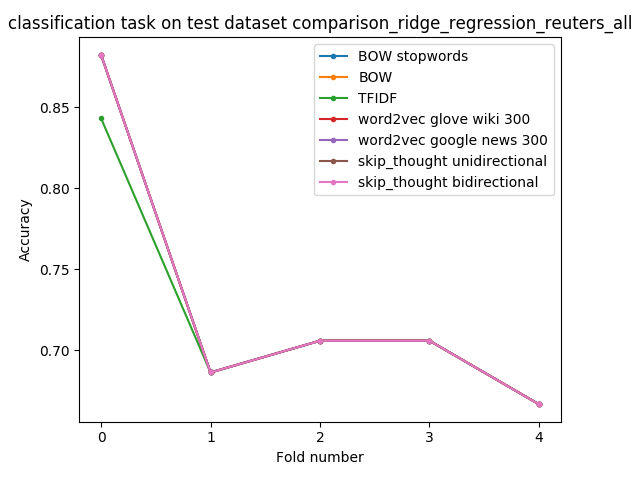
\includegraphics[width=\linewidth]{../../picture/experiment/classification_test_comparison_ridge_regression_reuters_all.png}
  \caption{Classification task on Reuters testing data using Ridge regression}
  \label{fig:re_cls_all}
\end{figure}

\subsection{Models comparison}
We exam the performance using different models in Figure \ref{fig:web_tr_cls_bow}, \ref{fig:web_cls_bow}, \ref{fig:re_tr_cls_bow} and \ref{fig:re_cls_bow}. In Figure \ref{fig:web_tr_cls_bow}, SVR has the best performance. It may explain the reason to choose
SVR in AZFinText \cite{AZFinText}. However, the result is opposite on Reuters data as shown in Figure \ref{fig:re_tr_cls_bow} and \ref{fig:re_cls_bow}. Ridge regression performs stable among all case.

\begin{figure}
  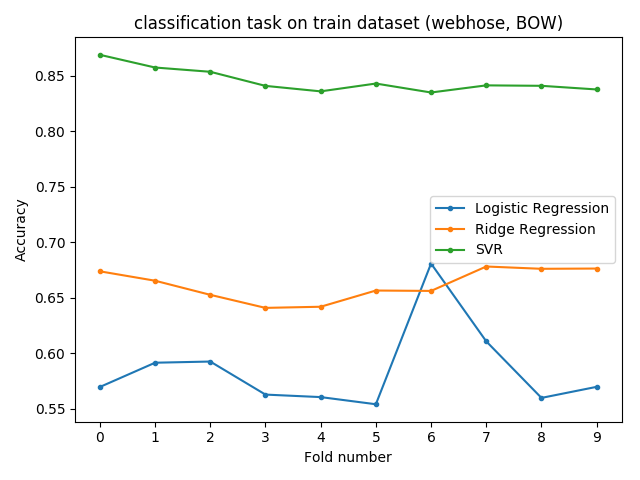
\includegraphics[width=\linewidth]{../../picture/experiment/classification_train_(webhose,_BOW).png}
  \caption{Classification task on Webhose.io training data with BOW features}
  \label{fig:web_tr_cls_bow}
\end{figure}

\begin{figure}
  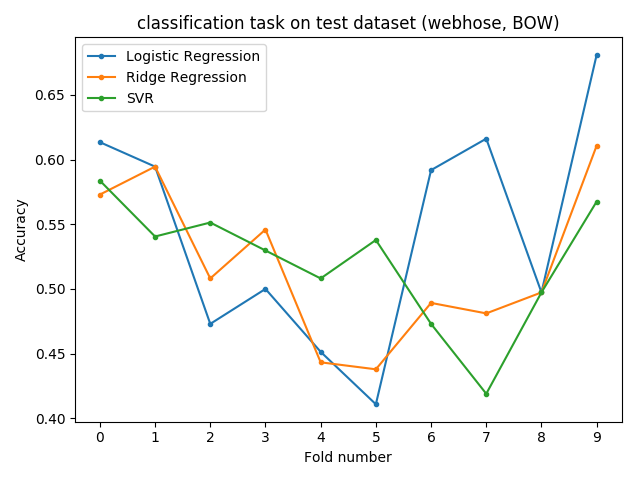
\includegraphics[width=\linewidth]{../../picture/experiment/classification_test_(webhose,_BOW).png}
  \caption{Classification task on Webhose.io testing data with BOW features}
  \label{fig:web_cls_bow}
\end{figure}

\begin{figure}
  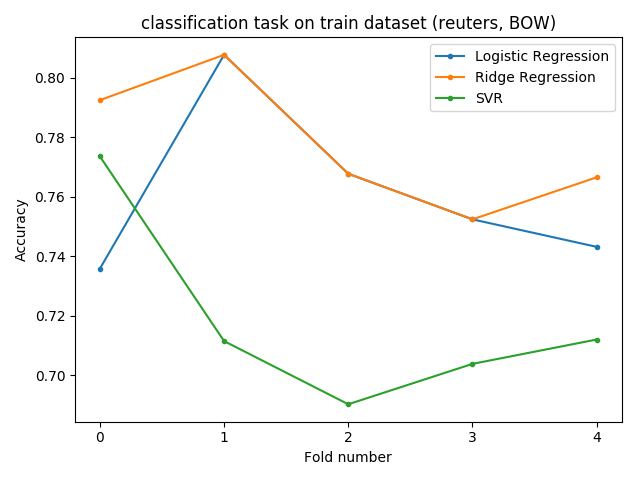
\includegraphics[width=\linewidth]{../../picture/experiment/classification_train_(reuters,_BOW).png}
  \caption{Classification task on Reuters training data with BOW features}
  \label{fig:re_tr_cls_bow}
\end{figure}

\begin{figure}
  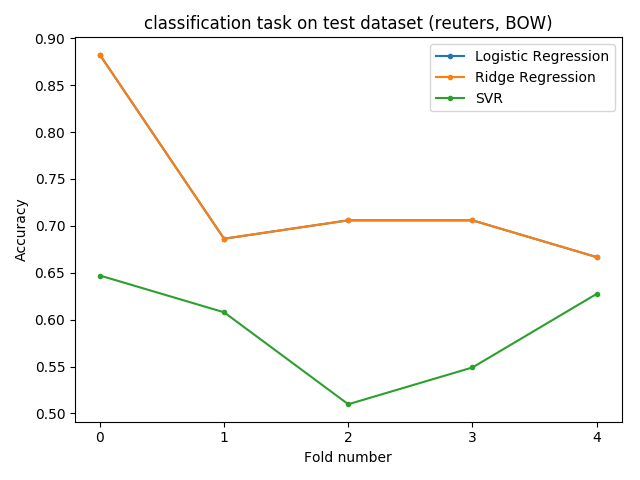
\includegraphics[width=\linewidth]{../../picture/experiment/classification_test_(reuters,_BOW).png}
  \caption{Classification task on Reuters testing data with BOW features}
  \label{fig:re_cls_bow}
\end{figure}

\subsection{Pos-tag filter comparison}
We exam the performance among different selected pos-tag filter in Figure \ref{fig:web_cls_tag} and \ref{fig:re_cls_tag}. The result shows choosing only proper noun has little difference with other bag-of-words features.
The good things for SVR and proper noun are that it is not easy to overfit. This is because the feature size is small by filtering out other terms.

\begin{figure}
  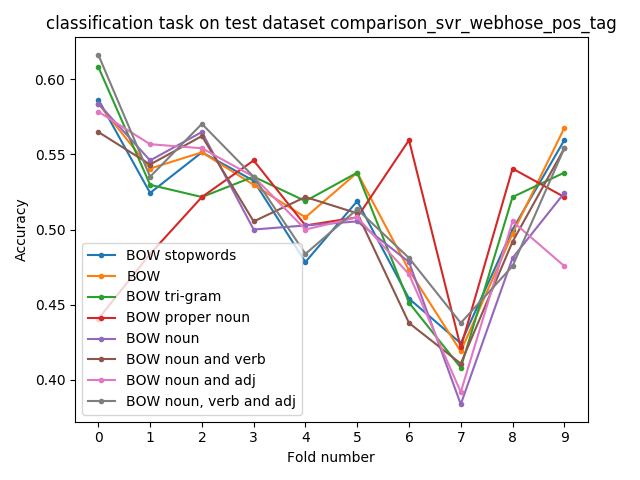
\includegraphics[width=\linewidth]{../../picture/experiment/classification_test_comparison_svr_webhose_pos_tag.png}
  \caption{Classification task on Webhose.io testing data using SVR with different pos-tag filter}
  \label{fig:web_cls_tag}
\end{figure}

\begin{figure}
  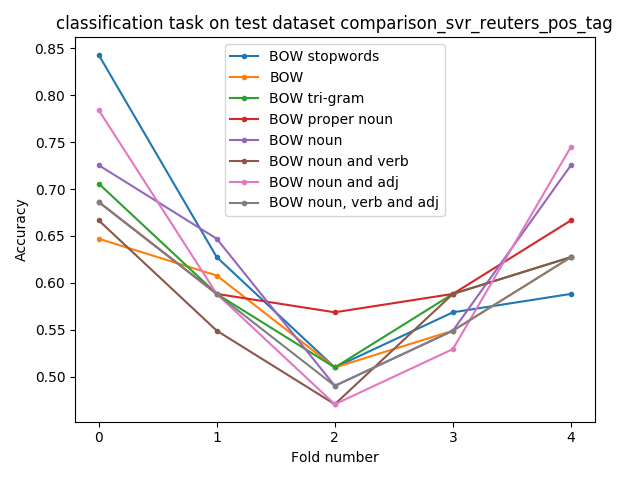
\includegraphics[width=\linewidth]{../../picture/experiment/classification_test_comparison_svr_reuters_pos_tag.png}
  \caption{Classification task on Reuters testing data using SVR with different pos-tag filter}
  \label{fig:re_cls_tag}
\end{figure}

\subsection{Trading}
Figure \ref{fig:re_pl_tag} shows the performance of trading using SVR and different pos-tag filter. We can find with only proper we can have profit in fold 3 (the only time we can gain among all models) but lose in fold 2.
However, since we don't have much data, we can not conclude the result in the long run.

\begin{figure}
  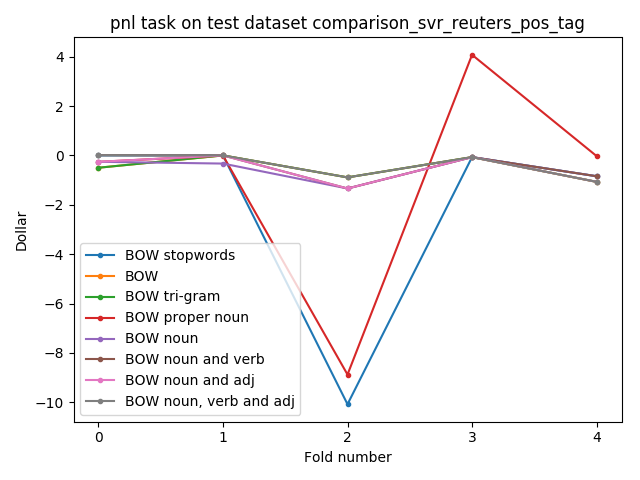
\includegraphics[width=\linewidth]{../../picture/experiment/pnl_test_comparison_svr_reuters_pos_tag.png}
  \caption{Trading task on Reuters testing data using SVR with different pos-tag filter}
  \label{fig:re_pl_tag}
\end{figure}

\section{Conclusion}
In this project, I crawled and built data pipeline for Webhose.io and Reuters datasets for stock price prediction using text features. Experiments are performed on three tasks and five different features to explore features
contributions on stock price prediction. Among all features, there is no significant difference in testing data. However, continuous text features have better generality than discrete features like bag-of-words. Among the different models,
ridge regression is the most stable one. We can not have any gain with the model. However, we could earn with SVR but lose money at a different time. Among all pos-tag filters, the difference is not huge. Selecting only
proper noun generates less feature size which is useful for avoiding overfitting. We also described why data qualities, insufficient data, various source, and ambiguous company identity, are still significant issues. Due to the inadequate
Reuters data, the trading experiment result cannot be concluded quickly. The only thing can say is the model is not likely to make money.


\bibliographystyle{ACM-Reference-Format}
\bibliography{citation} 
\end{document}
